%!TEX root = ../main.tex

\section{Appendix}
\label{sec:appendix}

In this section, we provide more concrete information about the evaluation part that have been conducted in our  work.
\subsubsection{Datasets.} The evaluation part of our work is conducted on different datasets. Below is more detail description of them.
\begin{itemize}
\item \textit{Freebase}: This is a huge knowledge graph consisting of general facts. To meet the requirement of running both rule mining and embedding, we adopt \textit{FB15K} \cite{Bordes:NIPS2013}, a dataset containing 15K entities, 1345 binary predicates and 592K binary facts.
\item \textit{Wikidata}: This is a free, community-based knowledge base maintained by the Wikimedia Foundation. In our experiments, our \textit{Wiki44K} dataset is created as subset of Wikidata dump from December 2014 by choosing triples that have entities appearing at least 20 times in the whole dataset, and then selecting top 100 predicates that have most number of facts. This result is a dataset with 250K binary facts over 44K entities and 100 relations.
\item \textit{IMDB}\footnote{http://www.imdb.com/}: We construct a domain-specific KG from \textit{IMDB} dataset, which is also used in \cite{trantowards}. The KG consists of 118K entities, 37 predicates and 301K are binary facts.
\end{itemize}
While we train embedding models on \textit{IMDB} without external text, these embedding models are trained on \textit{FB15K} and \textit{Wiki44K} with 2 different settings: with and without the external textual data. In particular, each entity of \textit{FB15K} and \textit{Wiki44K} is linked with a small piece of description text, which is extracted from the corresponding Wikidata page. Furthermore, we discard all entities having empty description text for both experiment's settings.

As mentioned in the evaluation part, we used these datasets as reference graphs $\cG^i_{appr}$ to approximate $\cG^i$. We then constructed $\G$ by randomly selecting $80\%$ of its facts while preserving the distribution of facts over predicates. Figure \ref{table:pred_distribution} demonstrates the distribution of facts over top 50 predicates for the 3 datasets.
 \begin{figure}[t]
     \centering
     \subfloat[FB15K]{{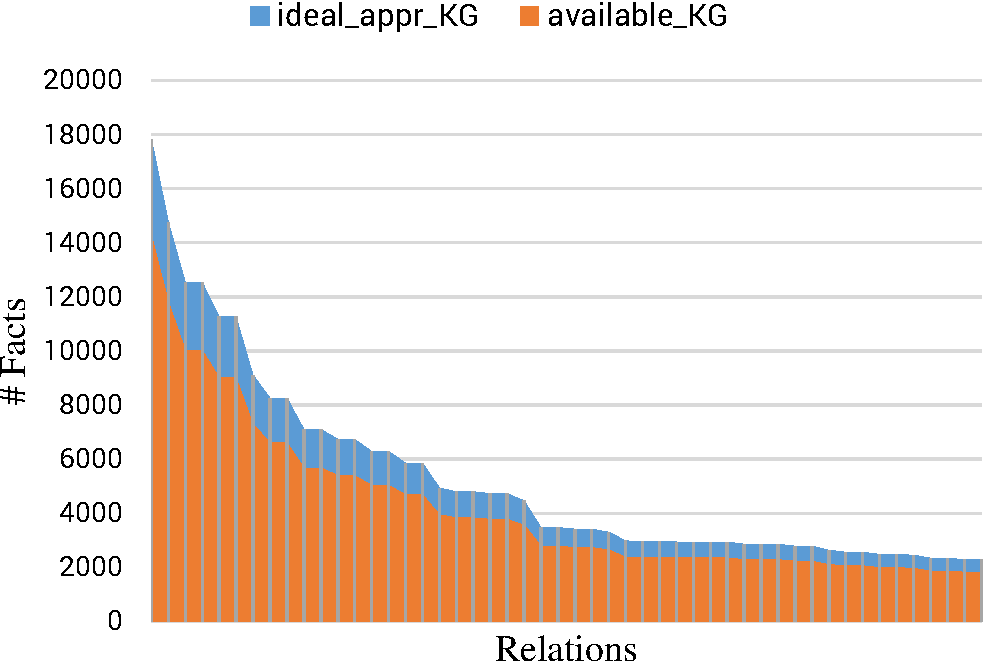
\includegraphics[width=0.5\textwidth]{figures/technical_rp/fb15k_pred_dist-crop.pdf} }}
     \subfloat[Wiki44K]{{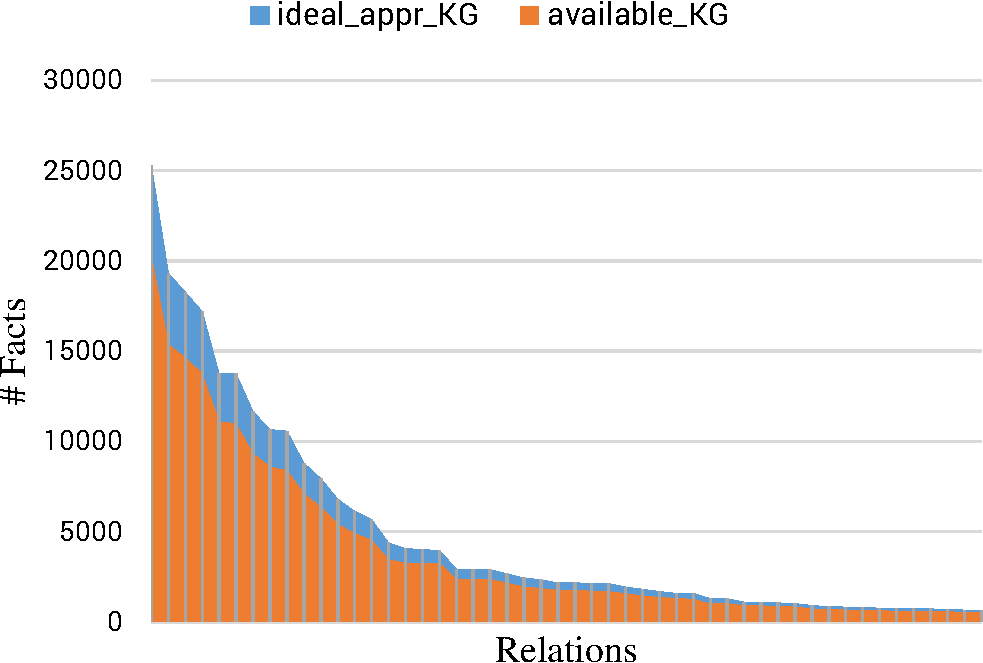
\includegraphics[width=0.5\textwidth]{figures/technical_rp/wiki44k_pred_dist-crop.pdf} }}\\
     \subfloat[IMDB]{{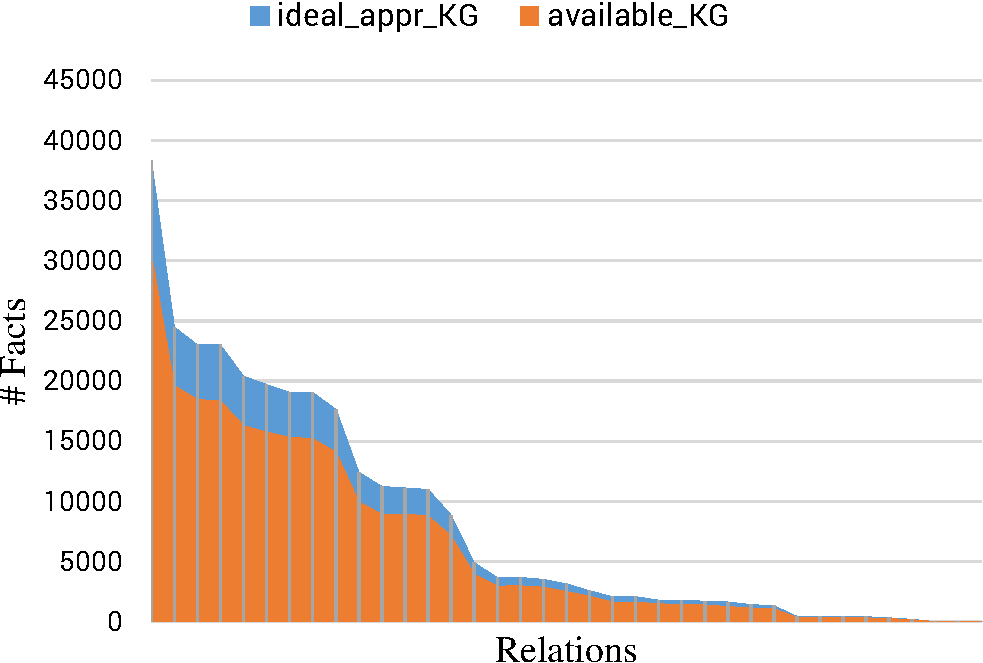
\includegraphics[width=0.5\textwidth]{figures/technical_rp/imdb_pred_dist-crop.pdf} }}
     \caption{Distribution of facts over top 50 relations of ideal approximation KG $\cG^i_{appr}$ and available KG $\cG$.}
     \label{table:pred_distribution}
\end{figure}

\begin{table}[h]
\centering
\begin{tabular}{ | l | l | } 
 \hline
 MODEL & NUMBER OF PARAMETERS \\ 
 \hline
 RESCAL\cite{conf/icml/NickelTK11} & $O(n_ek +n_rk^2)$    \\ 
 SE\cite{Bordes:2011:LSE:2900423.2900470} & $O(n_ek +2n_rk^2)$ \\ 
 SME(Linear)\cite{DBLP:journals/corr/abs-1301-3485} & $O(n_ek +n_rk +4k^2)$  \\ 
 SME(Bilinear)\cite{DBLP:journals/corr/abs-1301-3485} &  $O(n_ek +n_rk +2k^3)$ \\ 
 LFM \cite{Jenatton:2012:LFM:2999325.2999488} &  $O(n_ek +n_rk +10k^2)$ \\
 \hline
 TransE \cite{Bordes:NIPS2013} & $O(n_ek +n_rk)$  \\ 
 HolE\cite{DBLP:conf/aaai/NickelRP16} & $O(n_ek +n_rk)$  \\ 
 \hline
 SSP \cite{DBLP:conf/aaai/0005HMZ17} & $O(2n_ek +n_rk)$\\
 \hline
\end{tabular}
\newline
\caption{Numbers of parameters for some embedding models (Adapt from \cite{Bordes:NIPS2013}). $n_e$ and $n_r$ are the number of entities and binary predicates; $k$ is the embeddings dimension.}
\label{table:embedding_recap}
\vspace*{-3mm}
\end{table}
\leanparagraph{Embedding models}
Table \ref{table:embedding_recap} recaps some embedding models having been introduced in the literature and their memory complexity. TransE \cite{Bordes:NIPS2013} and HolE \cite{DBLP:conf/aaai/NickelRP16} are two state-of-the-art embedding models regarding the setting of no external data. Meanwhile, when talking about embedding models using additional texts, SSP \cite{DBLP:conf/aaai/0005HMZ17} plays an important part. Apart from prediction quality, these models also have a good running time and memory complexity. Hence, we choose them to evaluate our approach.
\begin{table}[t]
\scriptsize
\centering
\begin{tabular}{|l|r r|r r|r r|r r|} 
 \hline
 DATASET & \multicolumn{4}{|c|}{FB15K} & \multicolumn{4}{|c|}{WIKI44}\\
 \hline
 MODEL & \multicolumn{2}{|c|}{MRR}& \multicolumn{2}{|c|}{Hits@10(\%)} & \multicolumn{2}{|c|}{MRR}& \multicolumn{2}{|c|}{Hits@10(\%)} \\
 $Eval.\ setting$ & $Raw$ & $Filt.$ & $Raw$ & $Filt.$ & $Raw$ & $Filt.$ & $Raw$ & $Filt.$\\
 \hline
 TransE& 0.23 & 0.33 & 47.48 & 59.64 & 0.22 & 0.26 & 39.23 & 43.58\\
 HolE & 0.24 & 0.36 & 47.54 & 60.45& 0.14 & 0.18 & 24.54 & 28.38  \\
 SSP & 0.29 & \textbf{0.45}& 55.73 & \textbf{70.35}& 0.26 & \textbf{0.31} & 45.15 & \textbf{51.05} \\
 \hline
\end{tabular}
\caption{Performance of embedding models on the two data sets.}
\label{table:embedding_performance}
\vspace*{-3mm}
\end{table}

We train these embedding models on the available KG $\cG$ of these datasets until convergence using Stochastic Gradient Descent. For evaluation protocol of the embedding models, we use the same method as in HolE \cite{DBLP:conf/aaai/NickelRP16}. To validate and test the models, we sampled 2000 facts from $\cG^i_{appr} \setminus \cG$ into the validation set, and other 2000 facts into the test set. We report the Mean Reciprocal Rank and the percentage of Hit@10 in Table \ref{table:embedding_performance}. The optimal hyperparameters  of each model and dataset are figured out by doing grid search. We select the hyperparameters, which result in the highest MRR score with \textit{filtered} setting on the validation set. To get a better understanding about how the evaluation is performed, see \cite{DBLP:conf/aaai/NickelRP16}.

\subsection{Embedding-Based Hybrid Quality Function}
\begin{figure}[t]
     \centering
     \subfloat[Conf-TransE on IMDB]{{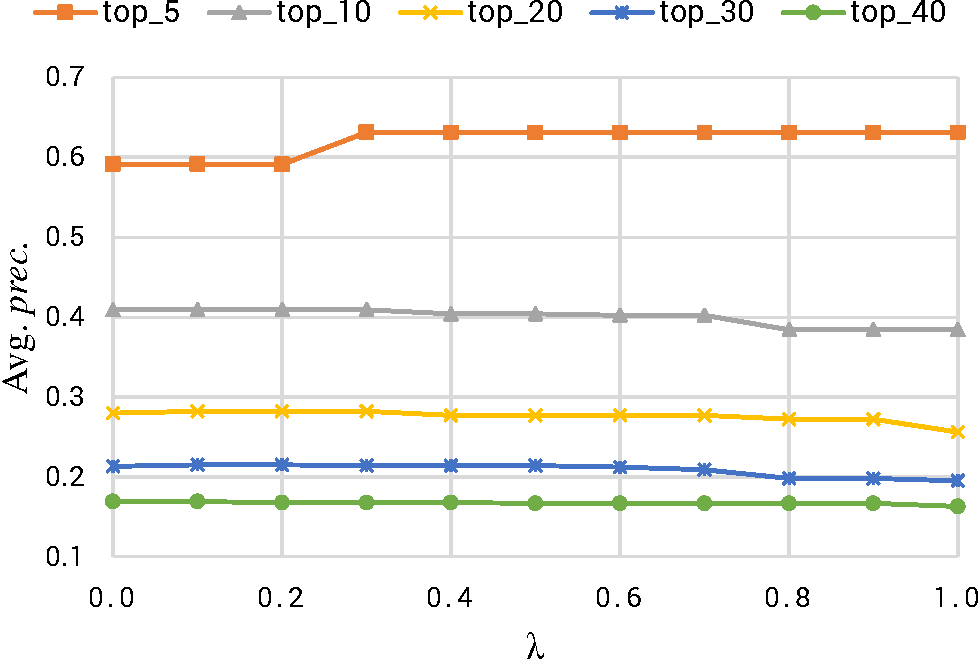
\includegraphics[width=0.5\textwidth]{figures/technical_rp/imdb_transe_conf-crop.pdf} }}
     \subfloat[Conv-TransE on IMDB]{{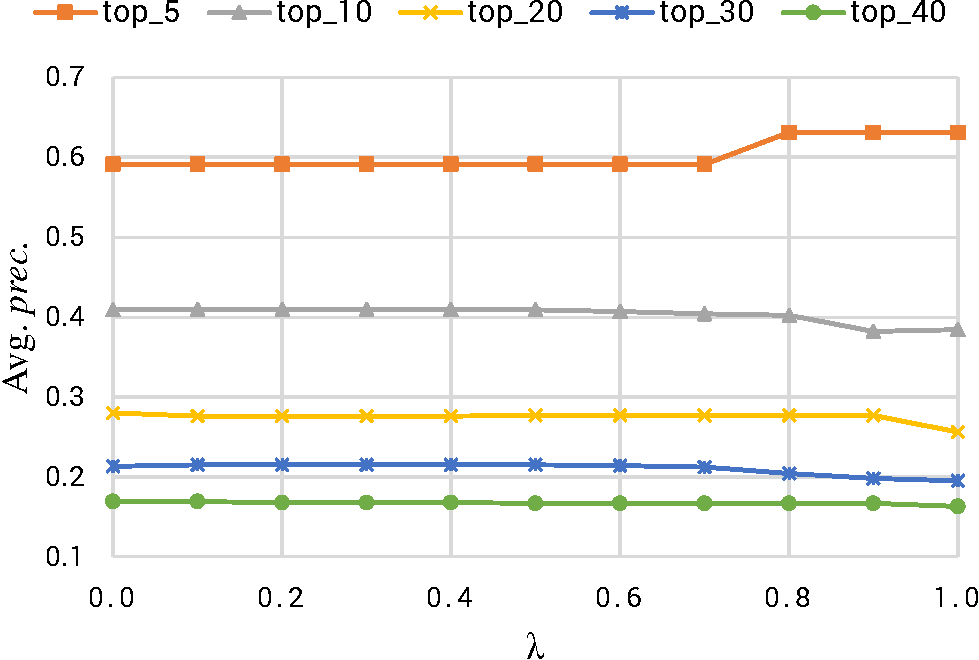
\includegraphics[width=0.5\textwidth]{figures/technical_rp/imdb_transe_conv-crop.pdf} }}\\
     \subfloat[PCA-TransE on IMDB]{{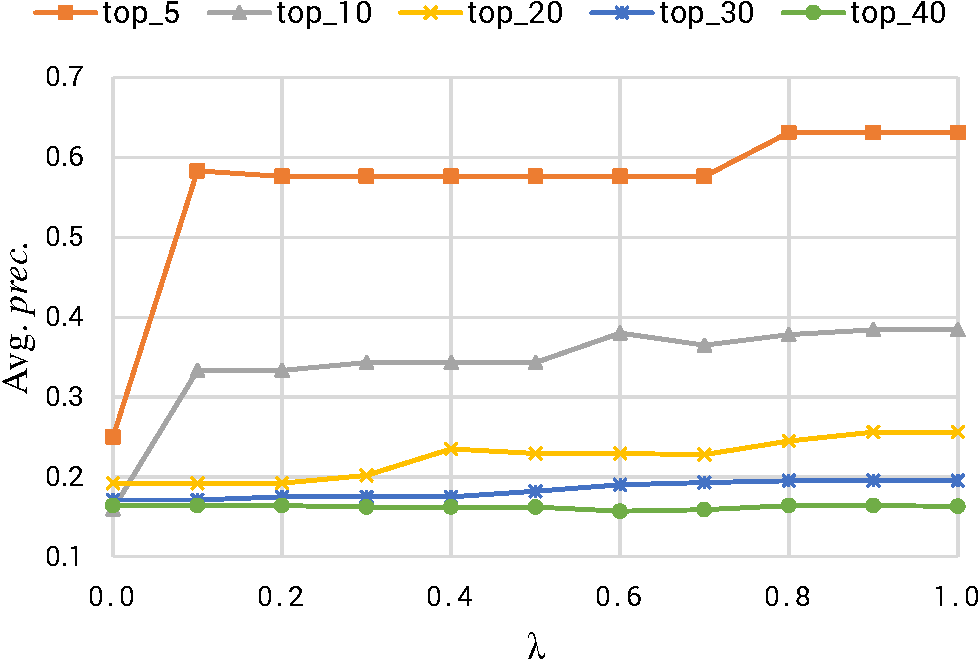
\includegraphics[width=0.5\textwidth]{figures/technical_rp/imdb_transe_pca-crop.pdf} }}
     \caption{$pred\_prec_{CW}$ of the \textit{top-k} rules with various \textit{embedding weights} on IMDB dataset.}
     \label{fig:appendix_exp1_imdb}
\end{figure}

Tables \ref{fig:appendix_exp1_imdb}, \ref{fig:appendix_exp1_fb15k}, \ref{fig:appendix_exp1_wiki44k} demonstrates the evaluation for experiment 1 for 3 mentioned datasets, with different configs, where we use $conf$, $conf_{pca}$ as $\mu_1$ and use TransE, HolE and SSP models to compute $\mu_2$. In addition, even though we require $\mu_1 \in [0,1]$, we also want to try one other metric, which does not hold this condition, to realize $\mu_1$. The metric we choose is $conviction$ \cite{trantowards}. Given $\mi{r:\; head\leftarrow body^+, not\;  body^-}$, conviction of $r$ is computed as follows:
\begin{align*}
\textit{conv}(r,\cG) & := \frac{1 - \textit{rel-supp}(head, \cG)}{1-\textit{conf}(r,\cG)}
\end{align*}
where $\textit{rel-supp}(head)$ is the relative support of the head, which is measured by:
\begin{align*}
\textit{rel-supp}(head, \cG) = \frac{|\set{(h, t) \mid head(h,t) \in \cG}|}{|\set{h \mid \exists t' \text{ s.t. }head(h,t') \in \cG}| \times |\set{t \mid \exists h'\text{ s.t. } head(h',t) \in \cG}|}
\end{align*}

We can see that with $conviction$, the best value of embedding weight $\lambda$ is close to 1. This is reasonable, since conviction could give us a value greater than 1. In addition, on \textit{IMDB} dataset, the usage of our hybrid quality measure does improve the quality of result. However, the improvement is not easily noticeable. One explanation is that this dataset is very spare, which could lead to the ineffectiveness of the embedding models.
\begin{figure}[t]
     \centering
     \subfloat[Conf-HoLE on FB15K]{{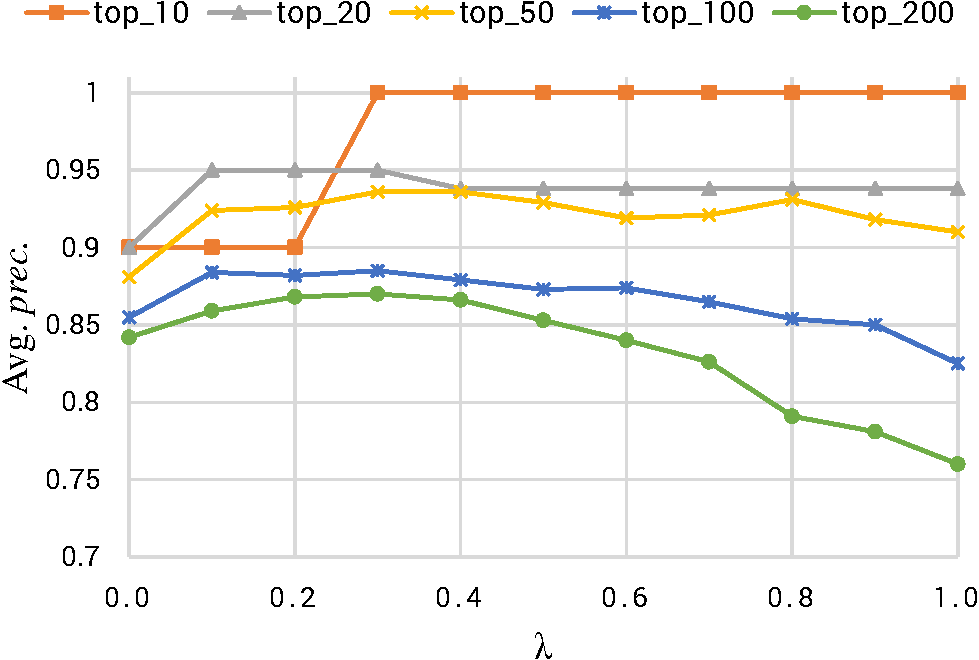
\includegraphics[width=0.5\textwidth]{figures/technical_rp/fb15k_hole_conf-crop.pdf} }}
     \subfloat[Conf-SSP on FB15K]{{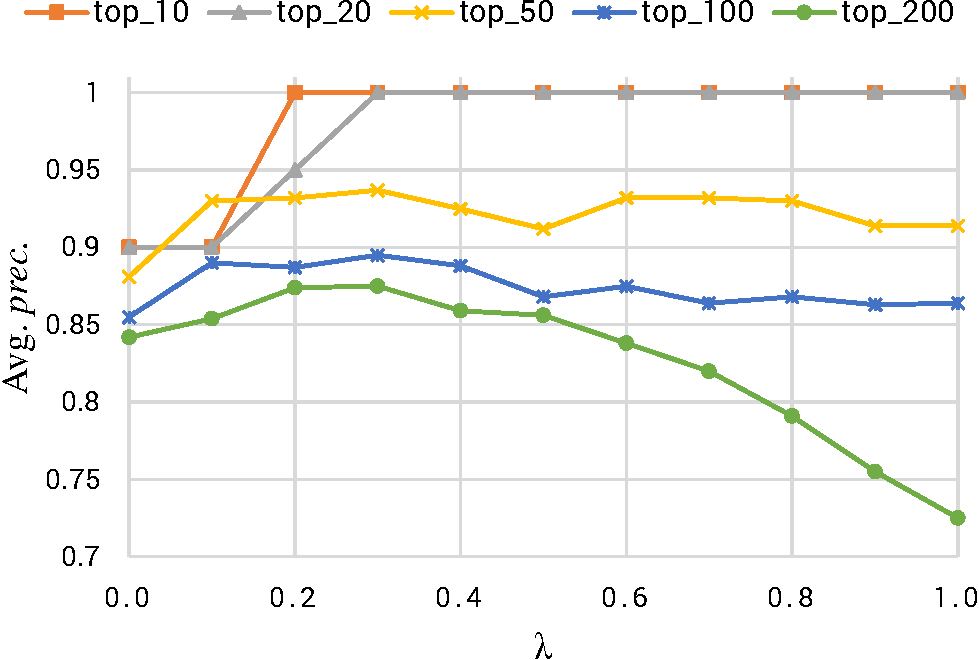
\includegraphics[width=0.5\textwidth]{figures/technical_rp/fb15k_ssp_conf-crop.pdf}}}\\
     \subfloat[PCA-HolE on FB15K]{{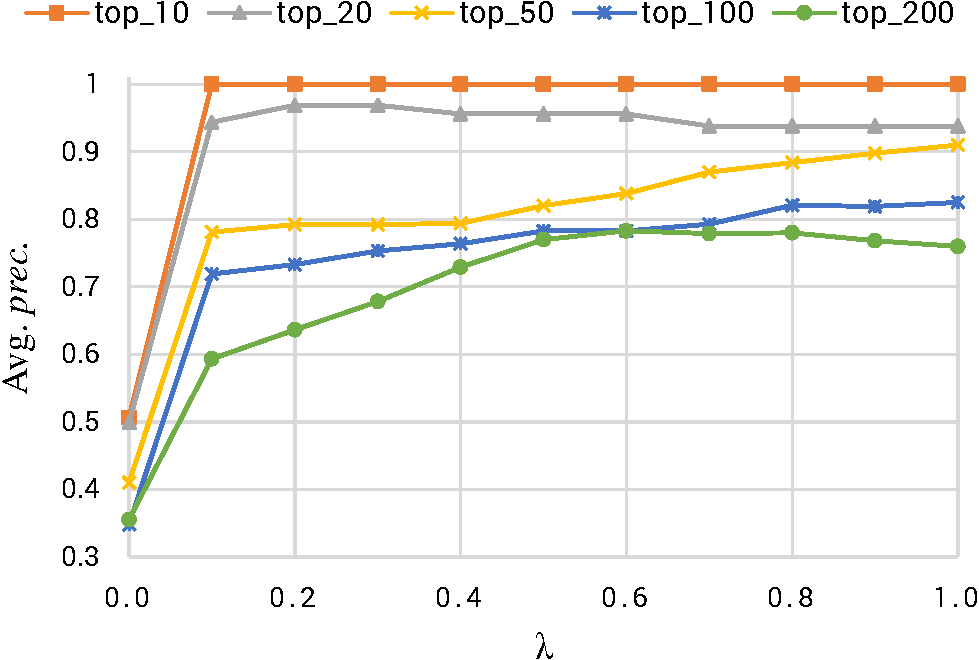
\includegraphics[width=0.5\textwidth]{figures/technical_rp/fb15k_hole_pca-crop.pdf} }}
     \subfloat[PCA-SSP on FB15K]{{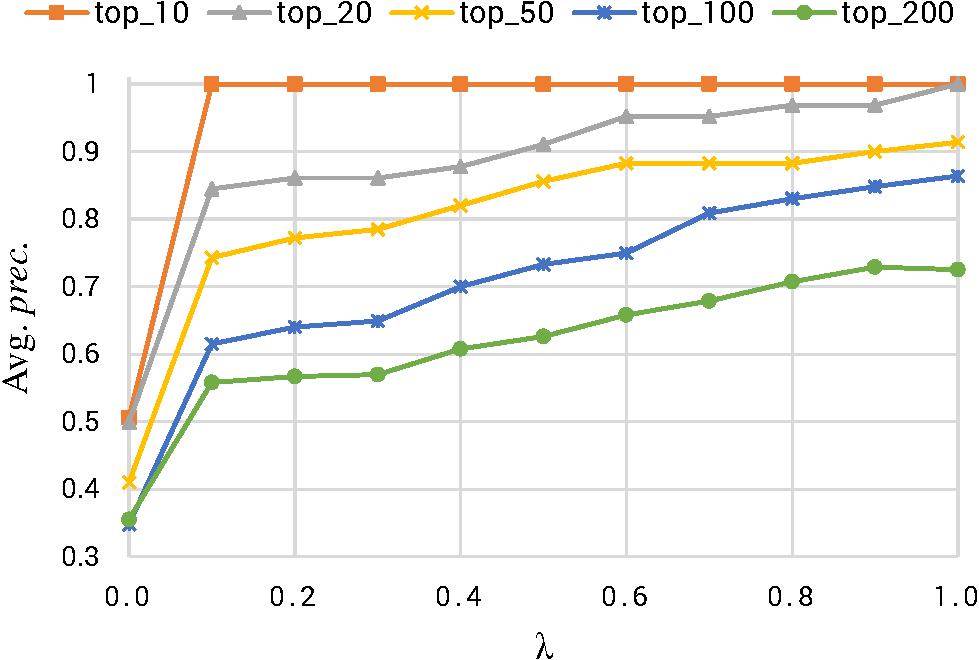
\includegraphics[width=0.5\textwidth]{figures/technical_rp/fb15k_ssp_pca-crop.pdf} }} \\   
     \subfloat[Conv-HolE on FB15K]{{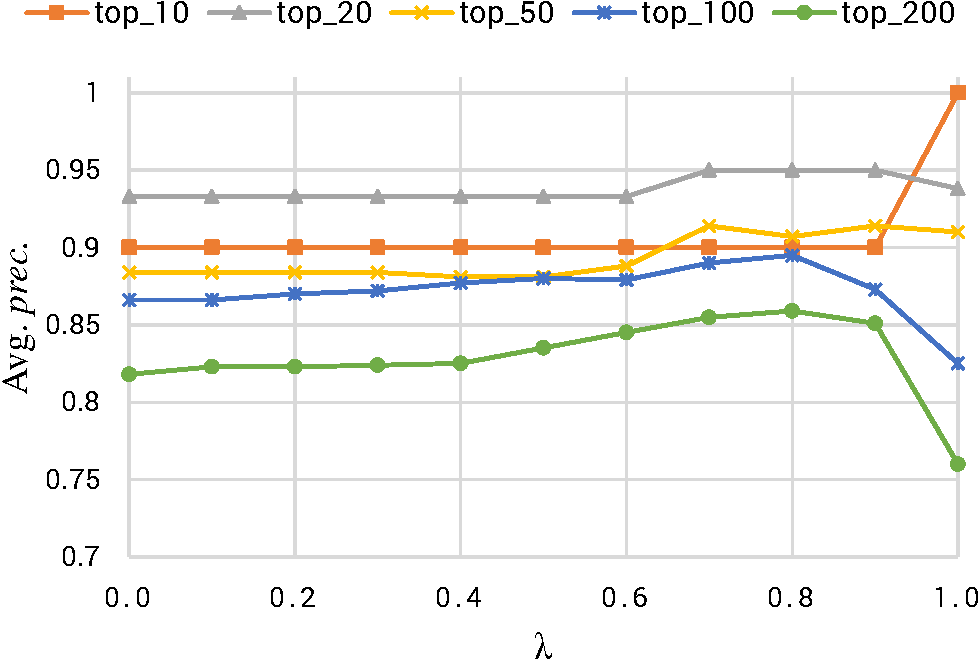
\includegraphics[width=0.5\textwidth]{figures/technical_rp/fb15k_hole_conv-crop.pdf} }}
     \subfloat[Conv-SSP on FB15K]{{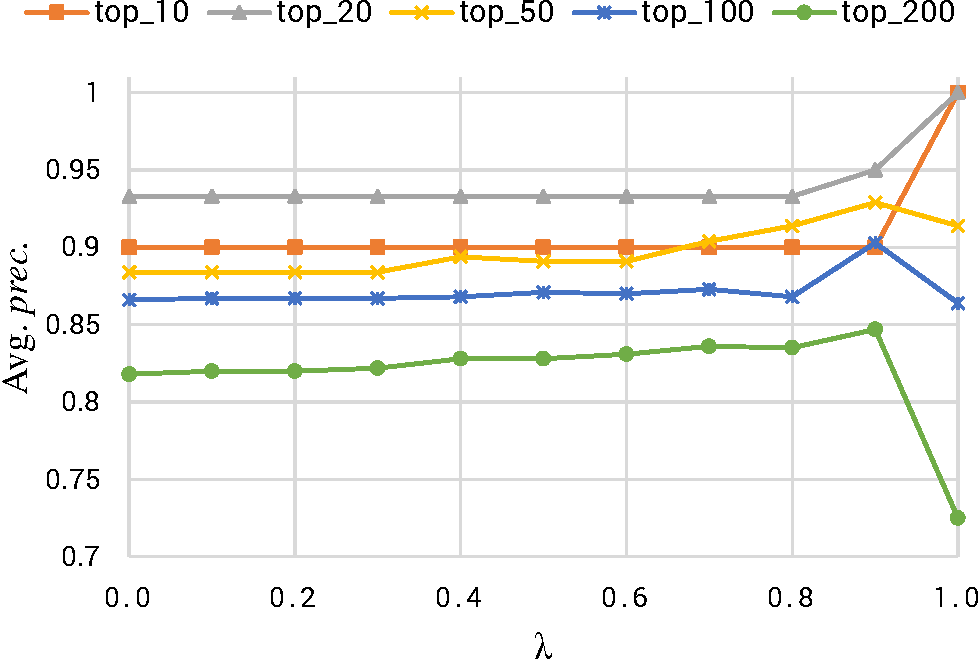
\includegraphics[width=0.5\textwidth]{figures/technical_rp/fb15k_ssp_conv-crop.pdf} }} \\   
     \caption{$pred\_prec_{CW}$ of the \textit{top-k} rules with various \textit{embedding weights} on FB15K dataset.}
     \label{fig:appendix_exp1_fb15k}
\end{figure} 
\begin{figure}[t]
     \centering
     \subfloat[Conf-TransE on Wiki44K]{{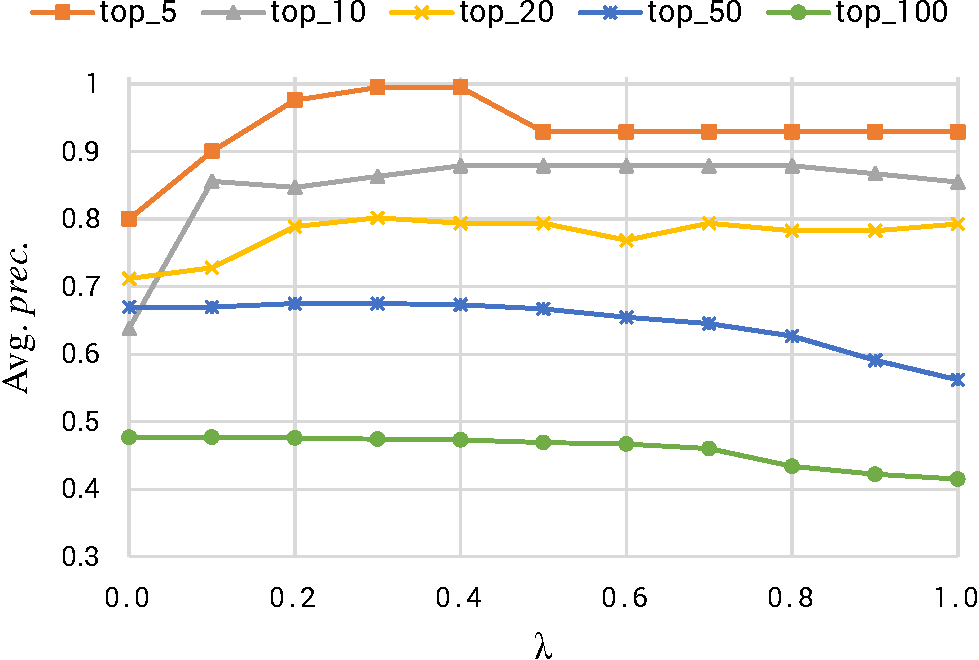
\includegraphics[width=0.5\textwidth]{figures/technical_rp/wiki44k_transe_conf-crop.pdf} }}
     \subfloat[Conf-SSP on Wiki44K]{{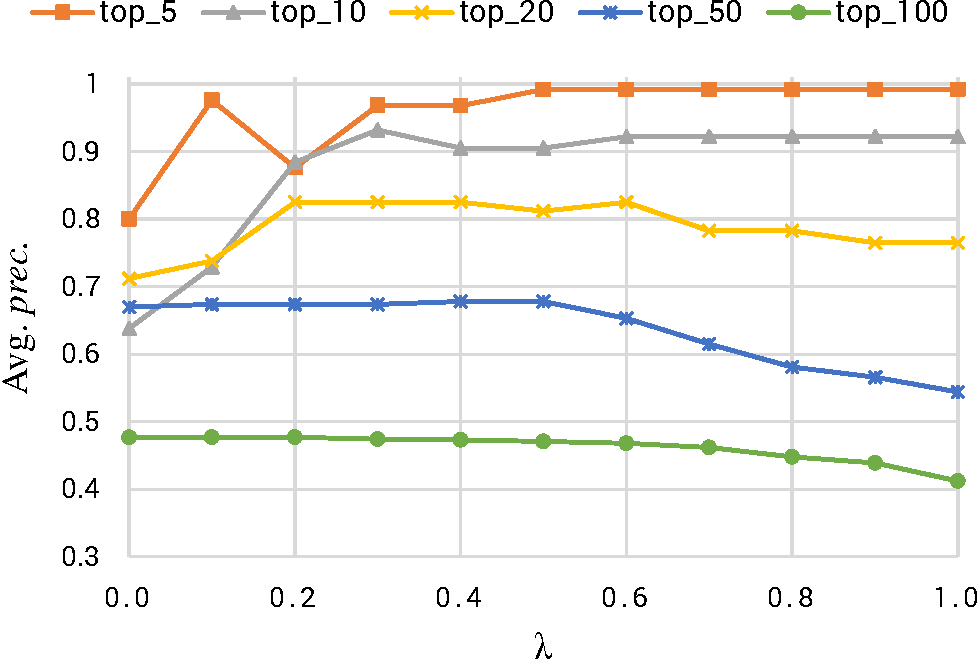
\includegraphics[width=0.5\textwidth]{figures/technical_rp/wiki44k_ssp_conf-crop.pdf}}}\\
     \subfloat[PCA-TransE on Wiki44K]{{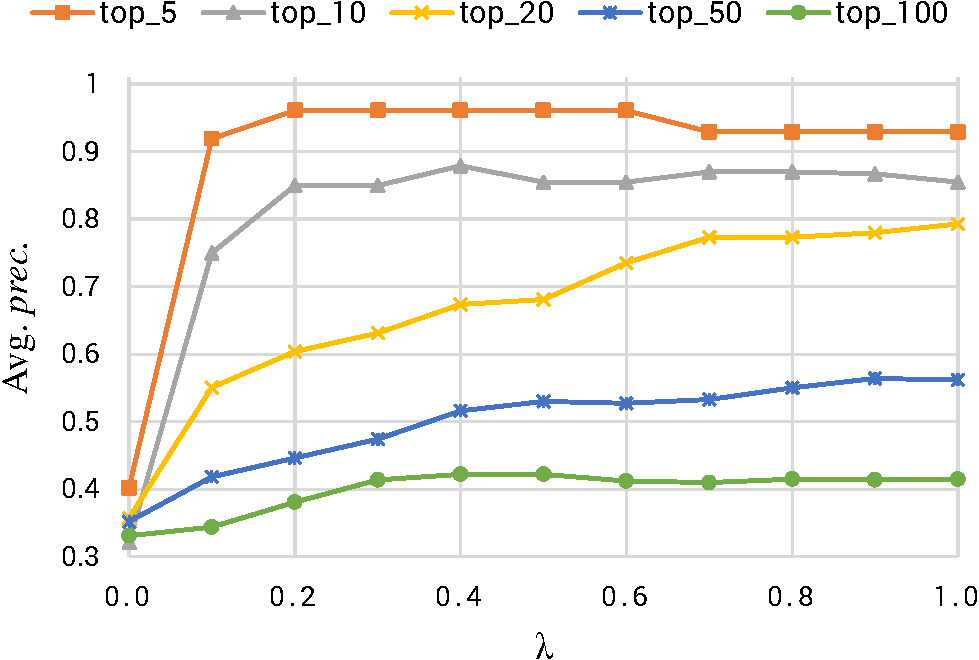
\includegraphics[width=0.5\textwidth]{figures/technical_rp/wiki44k_transe_pca-crop.pdf} }}
     \subfloat[PCA-SSP on Wiki44K]{{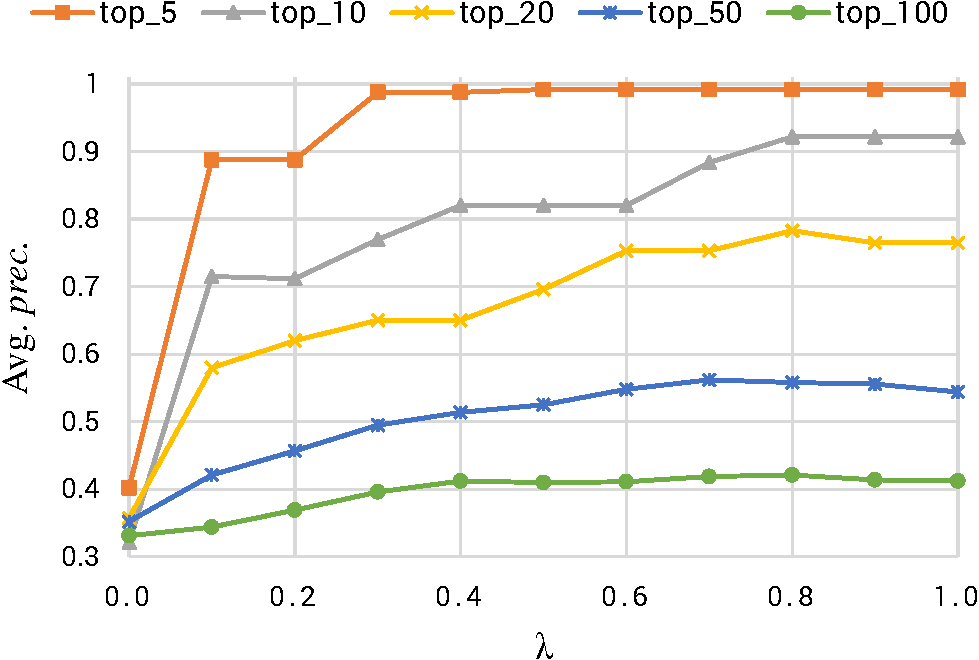
\includegraphics[width=0.5\textwidth]{figures/technical_rp/wiki44k_ssp_pca-crop.pdf} }} \\   
     \subfloat[Conv-TransE on Wiki44K]{{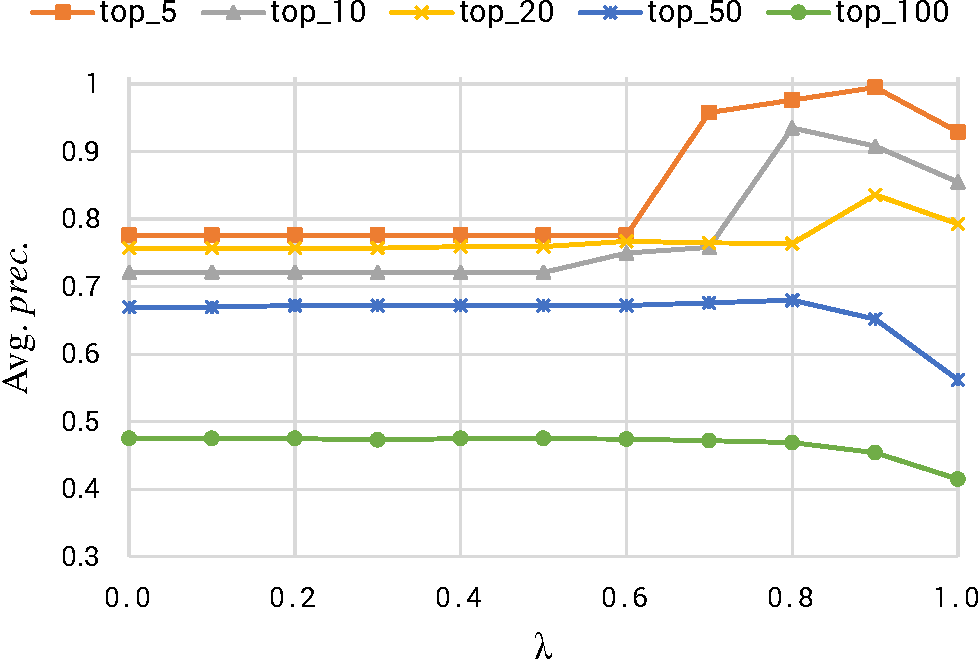
\includegraphics[width=0.5\textwidth]{figures/technical_rp/wiki44k_transe_conv-crop.pdf} }}
     \subfloat[Conv-SSP on Wiki44K]{{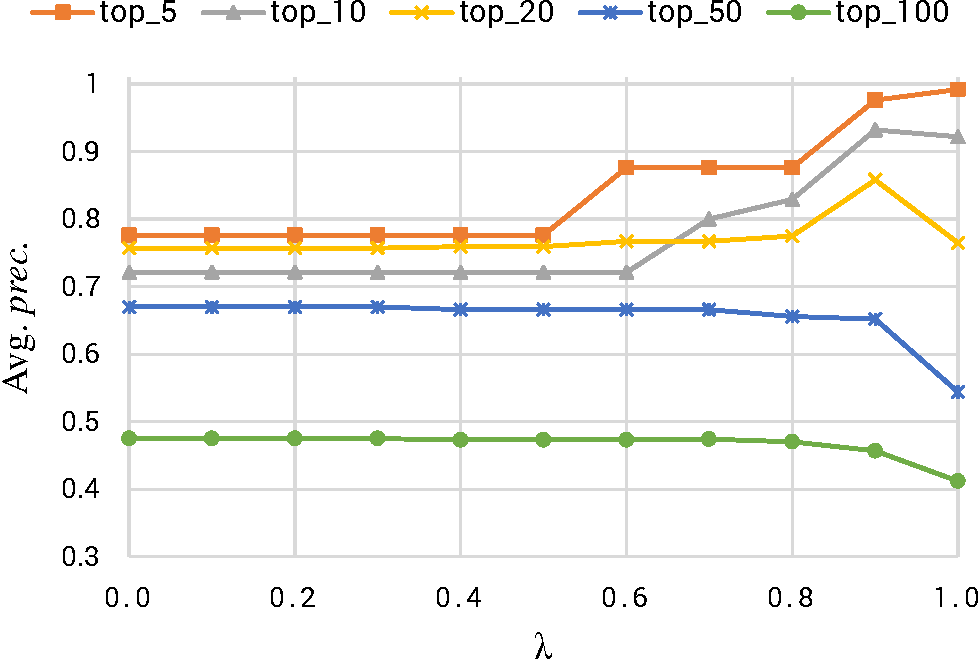
\includegraphics[width=0.5\textwidth]{figures/technical_rp/wiki44k_ssp_conv-crop.pdf} }}\\   
     \caption{$pred\_prec_{CW}$ of the \textit{top-k} rules with various \textit{embedding weights} on Wiki44K dataset.}
     \label{fig:appendix_exp1_wiki44k}
\end{figure} 

\begin{figure}[t]
     \centering
     \subfloat[FB15K]{{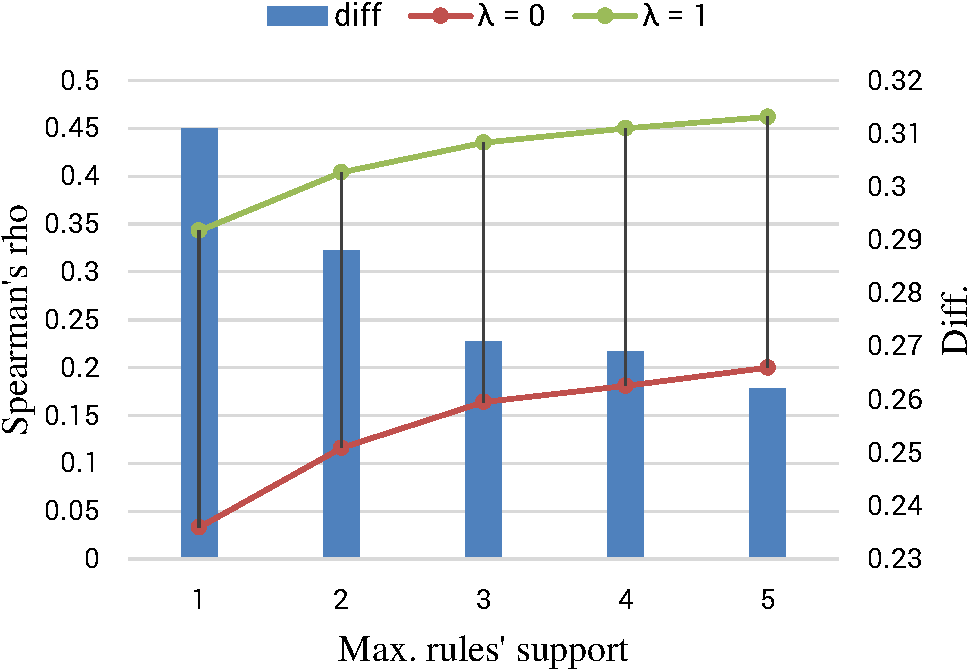
\includegraphics[width=0.5\textwidth]{figures/technical_rp/low_sp_fb15k-crop.pdf} }}
     \subfloat[Wiki44K]{{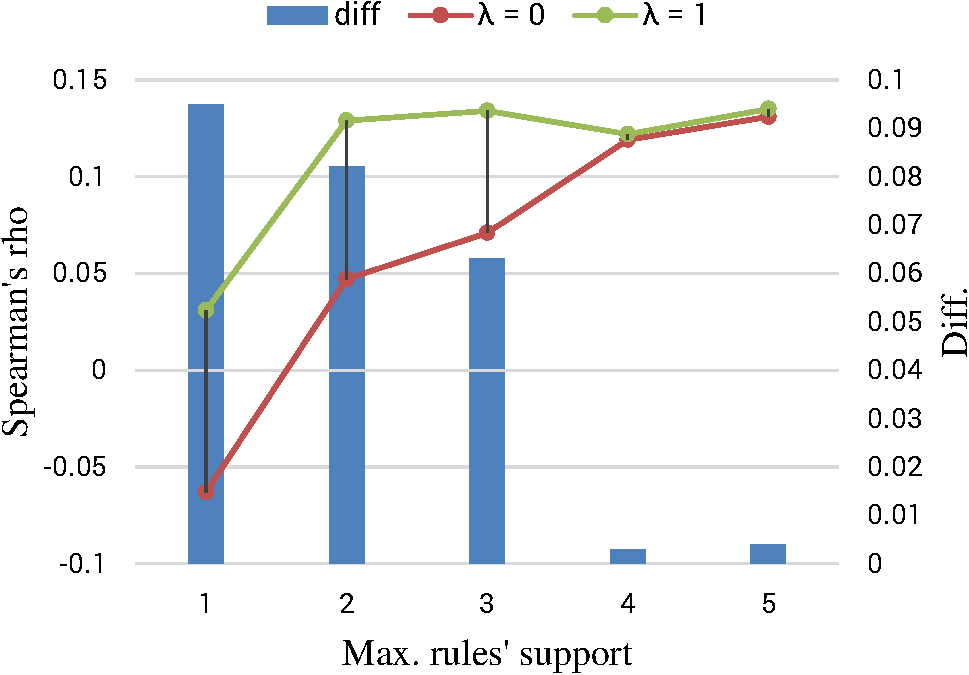
\includegraphics[width=0.5\textwidth]{figures/technical_rp/low_sp_wiki44k-crop.pdf} }}\\
     \subfloat[IMDB]{{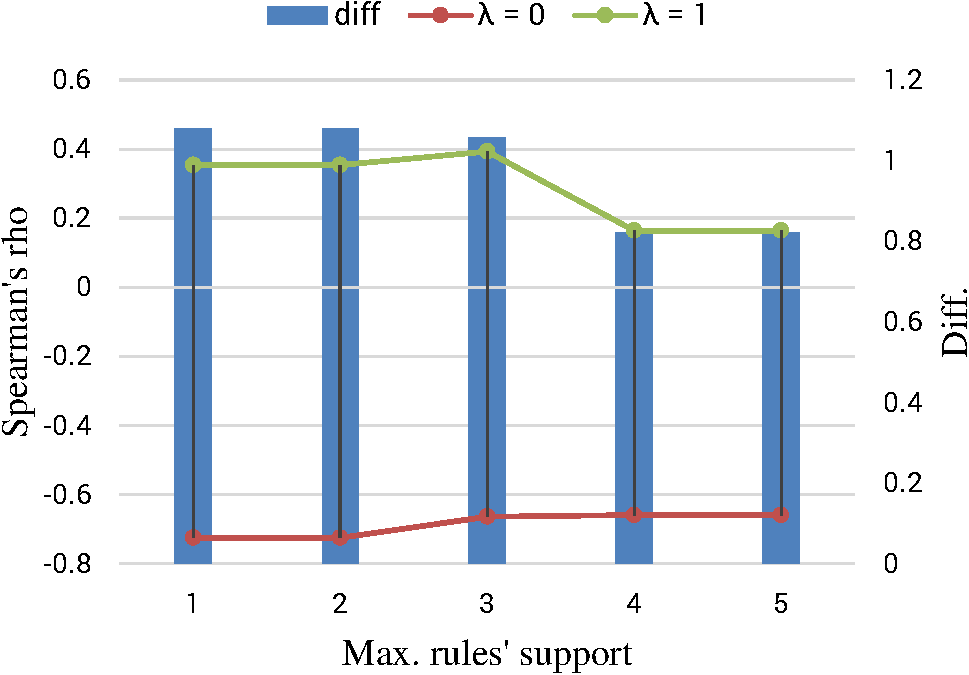
\includegraphics[width=0.5\textwidth]{figures/technical_rp/low_sp_imdb-crop.pdf} }}
     \caption{Spearman's rho of top rules ranked by confidence and the hybrid quality function, with limit on rules' support.}
     \label{fig:low_sp}
\end{figure}
\subsubsection{Handling rules with low support.}
One advantage of using the hybrid quality function comparing to standard rule measures (e.g. standard confidence) is at assessing rules having low support. In particular, when the rules have very low support, standard confidence is unreliable, since it estimates the rules' quality based on only a very small number of rules' instances. For example, ignoring all rules having confidence 1 since they do not infer any new facts, when a rule has support 1, its confidence is never greater than 0.5, even though the predicted facts may be good. 

Hybrid quality function $\mu$ fixes this issues by directly looking at the quality of predicted facts, which is achieved by feedback from the embedding models. We verify this hypothesis on \textit{FB15K}, \textit{Wiki44K} and \textit{IMDB} datasets. We also extracts rules of form $r:\;h(X,Z) \leftarrow p(X,Y), q(Y,Z)$ from $\cG$, with $conf(r,\cG) \geq 0.1$ and $\textit{r-supp}(r,\cG) \leq k$, where $k$ indicates the maximum support of rules to be extracted, we try different values of $k \in \{1,2,3,4,5\}$. These rules are then ranked using standard confidence itself ($\mu_1 = conf (\lambda = 0)$) and our hybrid quality function $\mu$. In addition, since we hypothesize that the confidence does not give strong information about the rules in this situation, we use $\mu = \mu_2 (\lambda = 1)$, where the hybrid quality function relies only on feedback from the embedding models. To compute $\mu_2$ in this case, we use the best embedding models for each dataset: SSP for \textit{FB15K}, \textit{Wiki44K} and TransE for \textit{IMDB}.

To evaluate the quality of the 2 ranked rule lists, we measure the Spearman's rank correlation coefficient of rules' confidence or hybrid quality with their $pred\_prec_{CW}$. Figure \ref{fig:low_sp} show the Spearman's rho of the 2 ranked lists and the difference of them with many values of rules support limit $k$. We can notice that the hybrid quality function outperforms standard confidence on all 3 datasets, and even works better with lower rule support.